\chapter{Introdução}

Aqui é a introdução da dissertação.

Vamos fazer algumas referências bibliográficas. O estilo a ser usado é o ABNT.

Artigo sem ano \citet{Longuet-1950}.\\
Em \citep{SPH_LIU_2003}
Em \cite{Scan-1990-Blelloch}

\section{Motivação}

Uma seção...

Agora vamos referenciar a Figura \ref{figuraEPS}.

\begin{figure}
   \begin{center}
     \scalebox{0.5}{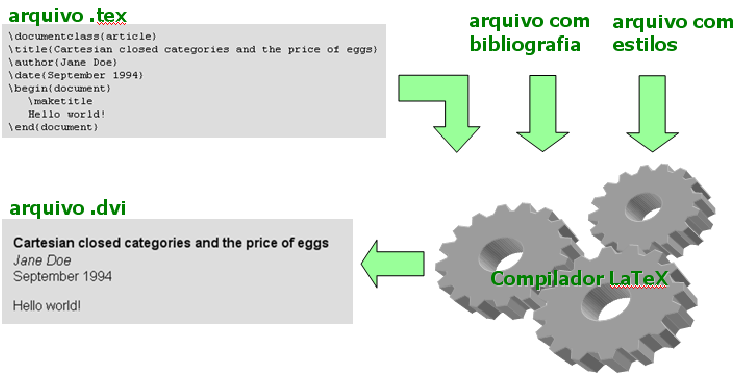
\includegraphics{figs/figuraTeste}}
   \end{center}
   \caption{Testando uma figura...\label{figuraEPS}}
\end{figure}


\subsection{Bla blá}

Uma subseção...

\subsubsection{ABC}

Uma subsub-seção.
